%----------------------------------------------------------------------------------------
%	PACKAGES AND OTHER DOCUMENT CONFIGURATIONS
%----------------------------------------------------------------------------------------

\documentclass[
11pt, % The default document font size, options: 10pt, 11pt, 12pt
oneside, % Two side (alternating margins) for binding by default, uncomment to switch to one side
%chapterinoneline,% Have the chapter title next to the number in one single line
spanish, % english
singlespacing, % Single line spacing, alternatives: onehalfspacing or doublespacing
%draft, % Uncomment to enable draft mode (no pictures, no links, overfull hboxes indicated)
%nolistspacing, % If the document is onehalfspacing or doublespacing, uncomment this to set spacing in lists to single
%liststotoc, % Uncomment to add the list of figures/tables/etc to the table of contents
%toctotoc, % Uncomment to add the main table of contents to the table of contents
%parskip, % Uncomment to add space between paragraphs
%nohyperref, % Uncomment to not load the hyperref package
headsepline, % Uncomment to get a line under the header
]{MastersDoctoralThesis} % The class file specifying the document structure

\usepackage[utf8]{inputenc} % Required for inputting international characters
\usepackage[T1]{fontenc} % Output font encoding for international characters

\usepackage{palatino} % Use the Palatino font by default

\usepackage[backend=bibtex,style=authoryear,natbib=true]{biblatex} % Use the bibtex backend with the authoryear citation style (which resembles APA)

\addbibresource{informe.bib} % The filename of the bibliography

\usepackage[autostyle=true]{csquotes} % Required to generate language-dependent quotes in the bibliography
\usepackage{blindtext}
\usepackage{enumitem}

%----------------------------------------------------------------------------------------
%	MARGIN SETTINGS
%----------------------------------------------------------------------------------------

\geometry{
	paper=a4paper, % Change to letterpaper for US letter
	inner=2.5cm, % Inner margin
	outer=3.8cm, % Outer margin
	bindingoffset=2cm, % Binding offset
	top=1.5cm, % Top margin
	bottom=1.5cm, % Bottom margin
	%showframe,% show how the type block is set on the page
}

%----------------------------------------------------------------------------------------
%	THESIS INFORMATION
%----------------------------------------------------------------------------------------

\thesistitle{Fine Food Reviews} % Your thesis title, this is used in the title and abstract, print it elsewhere with \ttitle
\supervisor{} % Your supervisor's name, this is used in the title page, print it elsewhere with \supname
\examiner{} % Your examiner's name, this is not currently used anywhere in the template, print it elsewhere with \examname
\author{Mauro Toscano(96890)\\Patricio Iribarne Catella(96619)\\Axel Lijdens (95772)} % Your name, this is used in the title page and abstract, print it elsewhere with \authorname
\addresses{} % Your address, this is not currently used anywhere in the template, print it elsewhere with \addressname

\subject{} % Your subject area, this is not currently used anywhere in the template, print it elsewhere with \subjectname
\keywords{} % Keywords for your thesis, this is not currently used anywhere in the template, print it elsewhere with \keywordnames
\university{FIUBA} % Your university's name and URL, this is used in the title page and abstract, print it elsewhere with \univname
\department{} % Your department's name and URL, this is used in the title page and abstract, print it elsewhere with \deptname
\group{TeamName (Kaggle)} % Your research group's name and URL, this is used in the title page, print it elsewhere with \groupname
\faculty{} % Your faculty's name and URL, this is used in the title page and abstract, print it elsewhere with \facname

\hypersetup{pdftitle=\ttitle} % Set the PDF's title to your title
\hypersetup{pdfauthor=\authorname} % Set the PDF's author to your name
\hypersetup{pdfkeywords=\keywordnames} % Set the PDF's keywords to your keywords

\begin{document}
\begin{otherlanguage}{spanish}

\frontmatter % Use roman page numbering style (i, ii, iii, iv...) for the pre-content pages

\pagestyle{plain} % Default to the plain heading style until the thesis style is called for the body content

%----------------------------------------------------------------------------------------
%	TITLE PAGE
%----------------------------------------------------------------------------------------

\begin{titlepage}
\begin{center}

{\scshape\LARGE \univname\par}\vspace{1.5cm} % University name
\textsc{\Large 7506 - Organizaci\'on de datos}\\[0.5cm] % Thesis type

\HRule \\[0.4cm] % Horizontal line
{\huge \bfseries \ttitle\par}\vspace{0.4cm} % Thesis title
\HRule \\[1.5cm] % Horizontal line

\begin{minipage}[t]{0.4\textwidth}
\begin{flushleft} \large
\emph{Author:}\\
\authorname % Author name - remove the \href bracket to remove the link
\end{flushleft}
\end{minipage}
\begin{minipage}[t]{0.4\textwidth}
\begin{flushright} \large
\emph{Supervisor:} \\
\supname % Supervisor name - remove the \href bracket to remove the link
\end{flushright}
\end{minipage}\\[3cm]

\large \textit{Predecir el puntaje de los reviews en funcion de sus datos}\\[0.3cm] % University requirement text
\textit{in the}\\[0.4cm]

{\large \today}\\[4cm] % Date
%\includegraphics{Logo} % University/department logo - uncomment to place it

\vfill
\end{center}
\end{titlepage}


%----------------------------------------------------------------------------------------
%	LIST OF CONTENTS/FIGURES/TABLES PAGES
%----------------------------------------------------------------------------------------

\tableofcontents % Prints the main table of contents

%----------------------------------------------------------------------------------------
%	ABBREVIATIONS
%----------------------------------------------------------------------------------------

\begin{abbreviations}{ll} % Include a list of abbreviations (a table of two columns)

\textbf{DF} & \textbf{D}ata \textbf{F}rame\\
\textbf{DTM} & \textbf{D}ocument \textbf{T}erm \textbf{M}atrix\\
\textbf{CV} & \textbf{C}ross \textbf{V}alidation\\
\textbf{CNN} & \textbf{C}onvolutional \textbf{N}eural \textbf{N}etworks\\
\textbf{RNN} & \textbf{R}ecurrent \textbf{N}eural \textbf{N}etworks\\

\end{abbreviations}

%----------------------------------------------------------------------------------------
%	THESIS CONTENT - CHAPTERS
%----------------------------------------------------------------------------------------

\mainmatter % Begin numeric (1,2,3...) page numbering

\pagestyle{thesis} % Return the page headers back to the "thesis" style

% Include the chapters of the thesis as separate files from the Chapters folder
% Uncomment the lines as you write the chapters

% Chapter Template

\chapter{Introducci\'on} % Main chapter title

\label{Chapter1}

%----------------------------------------------------------------------------------------
%   SECTION 1
%----------------------------------------------------------------------------------------

\section{An\'alisis de los datos}

El trabajo consiste en desarrollar un algoritmo que permita predecir el puntaje (1-5) que un usuario
otorg\'o a un producto en base a su review (t\'itulo, texto, etc).

Para ello, vamos a hacer enfoque en el campo del ``sentiment analysis'', que consiste en poder
interpretar las emociones plasmadas en el texto.

Comenzamos utilizando algoritmos simples que nos permitieran hacer un an\'alisis r\'apido de los
datos, con el fin de poder estimar qu\'e tipos de algoritmos funcionan mejor, c\'omo preprocesar el
texto de forma que los resultados mejoren, etc.

%-----------------------------------
%   SUBSECTION 1
%-----------------------------------
\subsection{Preprocesamiento del set de entrenamiento}

Comenzamos por divir el set de entrenamiento en 3 partes:\\


\begin{itemize}
\setlength\itemsep{0em}
  \item train: consiste en un 80\% del set original. Es utilizado para entrenar los algoritmos.
  \item cv: consiste en un 10\% del set original. Es utilizado para ajustar los hiper par\'ametros de los
        algoritmos y reducir el overfitting al set de entrenamiento.
  \item test: consiste en el 10\% restante. Utilizado para evaluar el desempe\~no final del algoritmo.
\end{itemize}

De esta forma podemos tener una estimaci\'on confiable sobre los resultados obtenidos sin necesidad
de hacer varios submits a Kaggle.

%-----------------------------------
%   SUBSECTION 2
%-----------------------------------

\subsection{Preprocesamiento de los campos}

Cada review contiene una serie de campos con informaci\'on sobre el mismo:\\

\begin{itemize}
\setlength\itemsep{0em}
  \item Id - El id que identifica a cada review
  \item ProductId - El Id del producto
  \item UserId - El Id del usuario
  \item ProfileName - El nombre del usuario
  \item HelpfulnessNumerator - El numerador indicando la cantidad de usuarios que juzgaron al review como util
  \item HelpfulnessDenominator - El denominador indicando la cantidad de usuarios que evaluaron si el review fue útil o no
  \item Prediction - La cantidad de estrellas del review
  \item Time - Un timestamp para el review
  \item Summary - Un resumen del review
  \item Text - Texto del review
\end{itemize}

Encontramos que exceptuando Text y Summary, poco aportan los otros campos (y algunas veces hasta
entorpecen el aprendizaje).

%----------------------------------------------------------------------------------------
%   SECTION 2
%----------------------------------------------------------------------------------------

\section{Sentiment analysis}

Los puntajes otorgados a cada review se basan en que tan satisfechos estuvieron los usuarios con
el producto, por lo que los comentarios deber\'ian expresar cu\'al fue el sentimiento (alegr\'ia,
enojo, frustraci\'on, etc) al recibirlo.

Es por esto que consideramos que la finalidad de TP es, basicamente, hacer un sentiment analysis, y
luego mapear los sentimientos al valor del review.

En el sentiment analysis el preprocesamiento del texto juega un rol muy importante para la gran
mayor\'ia de los algoritmos \cite{importance_of_preprocessing}.

El primer paso es la tokenizaci\'on, que consiste en separar el texto en palabras u otros s\'imbolos
que puedan aparecer (URLs, emoticones, puntos, comas, tags HTML, etc) \cite{mining_twitter_data}.

Los emoticones son de suma importancia, por lo que, para evitar perderlos y poder
interpretarlos mejor, se pueden reemplazar por alguna palabra, por ejemplo:

\begin{itemize}
\setlength\itemsep{0em}
  \item :), :-) -> smile
  \item :( -> sad
\end{itemize}

Un paso bastante com\'un, es remover las llamadas ``stop words'', que son palabras muy comunes en
los textos, y por lo general no aportan mucho al significado general de la oraci\'on \cite{stopwords}.

Además, para facilitar el reconocimiento de las palabras, es \'util realizar un proceso conocido como stemming.
En \'este, se busca unificar todas las palabras que tengan un mismo origen o ra\'iz. Esto si bien nos hace perder informaci\'on,
también nos permite generalizar más facilmente.

Por ejemplo, si un cliente hablara de cómo llega su producto, quizás se refiera en estos reviews a la palabra ``shipping''. O quizás hable de que el barco llegó lento y mencione ``ship''. Si bien son distintas, tienen una raíz que podría ser ``ship''. Lo mismo sucede con conjugaciones de verbos. Si alguien menciona que disfrutó la comida puede usar cualquier tiempo verbal. ``Enjoy'' ``Enjoyed'' ``Enjoying'', y carece de sentido tratar cada palabra por separado. Los sexos en sustantivos, y otras formas lingüisticas también llevan a otros arboles de palabras, que todas refieren al mismo concepto, o a la misma raíz.

Es interesantes marcar que la raíz que usemos para agrupar, no tiene por qué ser necesariamente una palabra. Esto es útil porque en la práctica permite simplificar los algoritmos de stemming. \cite{word_stemming}

%----------------------------------------------------------------------------------------
%   SECTION 3
%----------------------------------------------------------------------------------------

\section{Expandiendo el set de datos}

Por lo general, obtener más datos ayuda a mejorar el desempe\~no del algoritmo. Si bien no es
trivial generar texto o modificar ejemplos para obtener nuevos, al considerar el problema como
sentiment analysis podemos utilizar alg\'un set de datos que tenga frases o palabras con un
sentimiento asociado y entrenar un algoritmo para que lo aprenda a detectar.

Luego, otro algoritmo puede interpretar esos sentimientos y transformarlos en un valor 1-5.
De esta forma podemos aprovechar una cantidad mayor de datos, agregando un paso intermedio. \cite{lexicons_db}

% Chapter Template

\chapter{Desarrollo} % Main chapter title

\label{Desarrollo} % Change X to a consecutive number; for referencing this chapter elsewhere, use \ref{ChapterX}

%----------------------------------------------------------------------------------------
%   SECTION 1
%----------------------------------------------------------------------------------------

\section{Algoritmos usados}

Para comenzar, se decidió hacer uso de algoritmos simples y ver el resultado obtenido para poder
compararlos y decidir cuál de todos profundizar.

Las pruebas se realizaron con los subsets obtenidos de dividir el set original, como se explicó en
la introducción.

%-----------------------------------
%   SUBSECTION 1
%-----------------------------------
\subsection{KNN}

Uno de los primeros algoritmos a evaluar fue KNN. Para calcular las distancias, se decidió encodear
los textos en un DTM utilizando una biblioteca de R \cite{dtm_for_sentiment_analysis}.

Previa a la creación de la matriz, se hizo una limpieza del texto, removiendo stop-words, puntuaciones
HTML, etc.

Se comenzó probando con una porción muy pqueña del set (5\%), y se incrementó el tamaño en las pruebas
subsiguientes.

Al llegar a aproximadamente un 15\% del set, el algoritmo era demasiado lento para clasificar (algunas
horas), y no daba buenos resultados, por lo que se decidió probar otra alternativa.

Probablemente se pueda implementar mas adelante utilizando doc2vec, lo que debería reducir las
dimensiones de los textos, y además dar resultados más precisos debido a la natureleza de los
vectores generados (más similares al ser más parecidos).

%-----------------------------------
%   SUBSECTION 2
%-----------------------------------

\subsection{Random forest}

Este algritmo se comportó bastante mejor que KNN, ya que su tiempo de entrenamiento/clasificación
era muy inferior, pero los resultados no fueron demasido buenos para predecir calificaciones menores
a 3. 

Si bien la idea fue tomada de \cite{random_forest_movie_reviews}, se convirtieron los textos a un
bag of words y luego se la utilizó para entrenar el forest.

Se puede analizar más adelante aplicar una técnica similar a la del artículo citado.

% Chapter Template

\chapter{Otras ideas} % Main chapter title

\label{other_ideas} % Change X to a consecutive number; for referencing this chapter elsewhere, use \ref{ChapterX}

%----------------------------------------------------------------------------------------
%   SECTION 1
%----------------------------------------------------------------------------------------

\section{Motivaci\'on}

Algunas ideas que no se llegaron a implementar, pero que se van a probar mas adelante, son mezcla
de algoritmos que se encontraron en internet o papers, y que dieron buenos resultados.

Algunos son un poco complejos de implementar bien (o ajustar), por lo que se ir\'an investigando
de a poco.

%-----------------------------------
%   SUBSECTION 1
%-----------------------------------

\subsection{NN}

Teniendo en cienta que lo que buscamos es ``transformar'' el sentimiento del usuario en una
puntuaci\'on, se podr\'ia aplicar alg\'un algoritmo que transforme oraciones o palabras en una
interpretaci\'on de sentimientos, por ejemplo\\

    la peor experiencia de mi vida
    0   -5       0       0  0   2

siendo los numeros negativos cuando el sentimiento es negativo, y positivo de otra forma.

Luego una red neuronal podr\'ia interpretar luego las combinaciones de dichos sentimientos y obtener
un valor final.

%-----------------------------------
%   SUBSECTION 2
%-----------------------------------
\subsection{CNN}

Una posible soluci\'on seria utilizar CNN. La raz\'on es que debido al uso de feature maps, podr\'ian
lograr una buena interpretaci\'on de las palabras en sus contextos y aprender ciertos patrones que
derivan expresan el puntaje que otorgar\'ia el usuario, sin importar la ubicaci\'on de los mismos
en el texto.

El \'unico problema ser\'ia lidiar con una cantidad de entradas variable (cada texto tiene un largo)
distinto. Algunas opciones para esto son:

\begin{itemize}
\setlength\itemsep{0em}
   \item tomar el texto mas largo del set de entrenamiento y utilizarlo como valor m\'aximo (y luego
         paddear los textos mas cortos y recortar los mas largos)
   \item hacer ``wrap around''
   \item utilizar alguna herramienta como ``Doc2Vec'' para convertir los textos a vectores. \cite{doc2vec}
\end{itemize}

Los textos se pueden ingresar a la red en forma de bytes (caracter por caracter) o en alguna
representaci\'on distinta, por ejemplo, vectores obtenidos por ``word2vec'', una conversi\'on mas
simple de valores que indican el sentiemiento de cada palabra, etc. \cite{CNN_for_nlp}

%-----------------------------------
%   SUBSECTION 3
%-----------------------------------

\subsection{RNN}

Las RNN tienen la ventaja de poder trabajar con entradas de tama\~no variable, y poder recordar
contextos de manera m\'as inteligente que las CNN. Es por esto que se va a intentar probar de
implementar una para realizar el sentiment analysis. \cite{LSTM_sentiment_analysis}

%\include{Chapters/Chapter4}
% Chapter Template

\chapter{Modelo con LSTM} % Main chapter title

\label{LSTM} % Change X to a consecutive number; for referencing this chapter elsewhere, use \ref{ChapterX}

%----------------------------------------------------------------------------------------
%   SECTION 1
%----------------------------------------------------------------------------------------

\section{Herramientas}

Para desarrollar la implementaci\'on con LSTM se utiliz\'o el framework en python llamado Keras, que
implementa abstracciones sencillas para crear modelos de redes con distintas capas, utilizando
Tensorflow o Theano.

Si bien permite realizar desarrollos y pruebas de forma r\'apida, no tiene el nivel de ajuste tan
bajo nivel como utilizar directamente Theano o Tensorflow.

Todos los modelos fueron entrenados monitoreando el MSE (y la precisi\'on en los modelos por
clasificaci\'on), al mismo tiempo que se verificaba el ``desempe\~no'' en el set de cross-validation
para controlar el overfitting.

\begin{figure}[h]
    \centering
    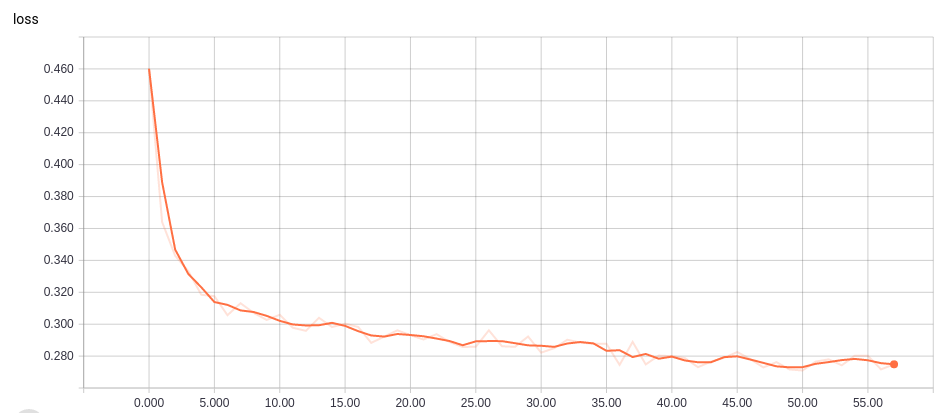
\includegraphics[width=1\linewidth]{Figures/train_loss.png}
    \decoRule
    \caption[Train loss]{El valor del costo en el entrenamiento.}
    \label{fig:Costo durante el entrenamiento}
\end{figure}

\begin{figure}[h]
    \centering
    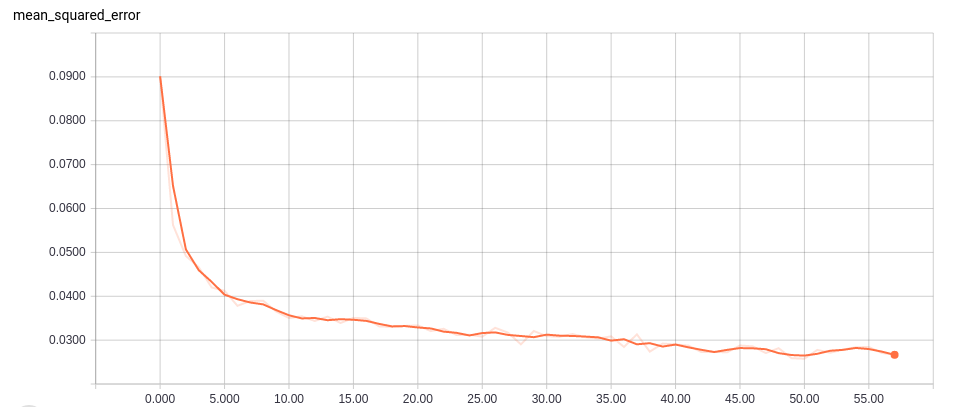
\includegraphics[width=1\linewidth]{Figures/train_mse.png}
    \decoRule
    \caption[MSE]{El valor del MSE en el set de entrenamiento.}
    \label{fig:MSE en el set de entrenamiento}
\end{figure}

\begin{figure}[h]
    \centering
    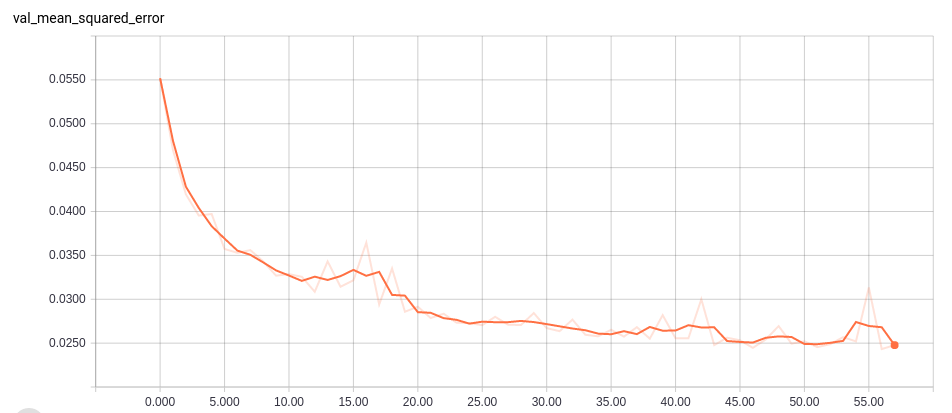
\includegraphics[width=1\linewidth]{Figures/val_mse.png}
    \decoRule
    \caption[Validation MSE]{El valor del MSE en el set de CV luego de cada iteraci\'on.}
    \label{fig:MSE en el set CV}
\end{figure}

%-----------------------------------
%   SUBSECTION 1
%-----------------------------------
\subsection{Limpieza del texto}

Como la cantidad de t\'erminos era enorme (alrededor de 100.000), realizamos un checkeo manual sobre
los textos, viendo que hab\'ia varias URLs, HTML, fechas, horas, comillas, etc. Esto resultaba en
una gran cantidad de tokens que realmente no aportaban demasiado, pero incrementaban el tama\~no de
los vectores encodeados, y por lo tanto  se decidi\'o hacer una limpieza del texto.

Las URLs fueron removidas, asi como tambi\'en el HTML y los separadores como ``---------''.
Las fechas y horas fueron reemplazadas por las palabras ``date'' y ``time'' respectivamente, as\'i
como los n\'umeros por la palabra ``number''. Las repeticiones del signo ``\$'' o los montos
``\$nnn'' fueron reemplazados por la palabra ``money''.

Tambi\'en se removieron las comillas alrededor de las citas, para evitar tokens del tipo `` 'this ''.

Otras pruebas r\'apidas llevaron a concluir que el texto en el campo `Summary' algunas veces
resultaba \'util, por lo que se decidi\'o incluirlo tambi\'en como parte del texto. Se experiment\'o
utilizando configuraciones de redes y entrenandolas con los sets que incluian o ignoraban los
summaries. Por lo general el resultado era mejor cuando se los incly\'o.

%-----------------------------------
%   SECTION 2
%-----------------------------------

\section{LSTM con 1-hot encoding}

Las redes LSTM mantienen un estado interno (``memoria'') lo que permite, a diferencia de las otras,
que la salida dependa no solo de la entrada, sino tambi\'en de las entradas anteriores
\cite{understanding_LSTM}. La forma de entrenarlas que utilizamos fue de a una palabra (encodeada
en un vector) a la vez.
Luego de analizar un review, el estado interno es reseteado. \cite{LSTM_time_series_predictions},
\cite{stateful_LSTM}

En todos los casos, se utiliz\'o entrenemiento por mini-batches para acelerar el proceso. Debido a
esto, hubo que seleccionar un valor fijo de t\'erminos por review.

\begin{figure}[h]
    \centering
    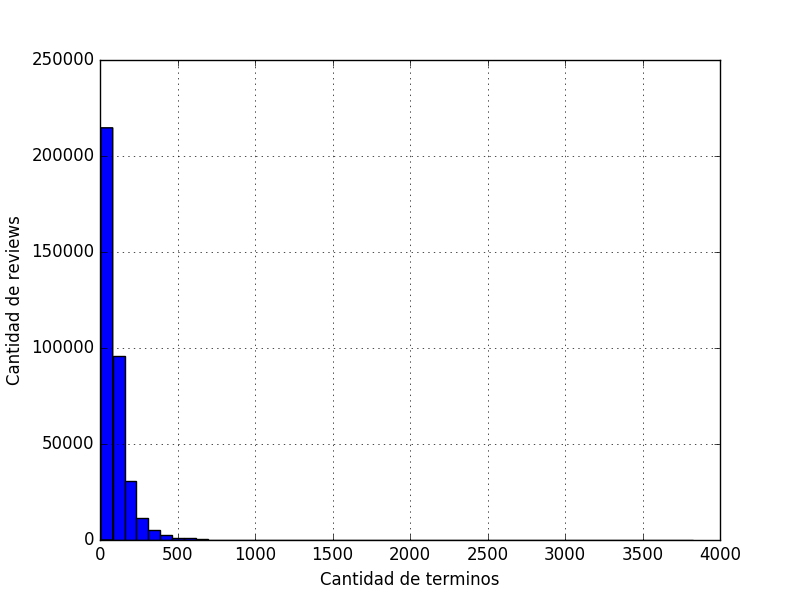
\includegraphics[width=1\linewidth]{Figures/terminos_por_review.png}
    \decoRule
    \caption[Terminos por review]{Histograma del largo de los reviews (por t\'erminos).}
    \label{fig:Histograma del largo de los reviews (por t\'erminos)}
\end{figure}

Debido a la cantidad de memoria requerida, no se pudo utilizar el largo mas grande (3826), por lo
que decidimos elegir 400, que abarcaba la gran mayoria. Los reviews de mayor longitud fueron
truncados, y los mas cortos paddeados con ceros al principio.

La primera prueba fue un modelo b\'asico que consis\'ia simplemente en 1 capa de 60 neuronas LSTM,
recibiendo las palabras en un 1-hot encoding, ignorando stop words. Este modelo ten\'ia 1 neurona
con funci\'on de activaci\'on sigmoidal como salida para obtener un resultado en el rango 0-1.

El modelo logr\'o un buen resultado para su simpleza (alrededor de 0.7 MSE en pruebas locales con el
set de cross-validation).

Agregando una capa m\'as de 60 neuronas LSTM, el MSE mejor\'o alrededor de un 0.1.

Paralelamente, los modelos equivalentes de clasificaci\'on (esto es, reemplazando la salida
sigmoidal por 5 neuronas softmax) daban resultados un poco peores. Es por esto que decidimos
enfocarnos m\'as en los modelos de regresi\'on, ya que los tiempos de entrenamiento eran de varias
horas.

%----------------------------------------------------------------------------------------
%   SUBSECTION 1
%----------------------------------------------------------------------------------------

\subsection{Aplicando capas convolucionales}

Como las palabras cambian su sentido en base al contexto, por lo general suele ser mejor aplicar
modelos de N-gramas.

Las redes convolucionales funcionan de manera similar, detectando patrones utilizando feature maps.
De esta forma, la red puede ``leer'' de a varias palabras, teniendo en cuenta el contexto de las
mismas \cite{text_classification_using_CNN}.

El siguiente modelo consisti\'o en agregar una capa convolucional con una de maxpooling como entrada
de la red. Como los resultados no mejoraron, probamos agregar varias capas con distintos tama\~nos
de filtros. Los resultados en este caso fueron levemente mejores, e incluso en Kaggle el score fue
de 0.4 aproximadamente.

%----------------------------------------------------------------------------------------
%   SECTION 3
%----------------------------------------------------------------------------------------

\section{Word2vec}

La siguiente prueba fue analizar si utilizando word2vec se podr\'ia lograr una mejora en el
algoritmo \cite{w2v_text_classification}.

La idea de utilizar word2vec es que las palabras con significados similares est\'an asociadas a
vectores cercanos, o que operaciones entre los mismos (suma, resta) resulta en vectores con cierto
sentido. Idealmente, si una palabra no fue vista en el set de entrenamiento pero en un sin\'onimo de
alguna que estaba presente, la red deber\'ia poder reconocerla igual.

Utilizando el modelo de word2vec de Google \cite{word2vec_google} como entrada a la red, se obtuvo
una leve mejora, aunque no fue f\'acil experimentar con los hiper-par\'ametros debido a los largos
tiempos de entrenamiento de la red (16 hs aproximadamente).

El modelo final consisti\'o en 3 capas convolucionales, con filtros de tama\~no 4, 5 y 6, yendo a
una capa de maxpooling, luego otra convolucional (esta vez con menos filtros), luego una capa LSTM
y finalmente se combinaron esas 3 capas mediante otra de LSTM (con la salida sigmoidal o softmax).


%----------------------------------------------------------------------------------------
%   SECTION 4
%----------------------------------------------------------------------------------------

\section{An\'alisis de los resultados}

Observando los resultados de las clasificaciones en el set de pruebas, se not\'o que la red ten\'ia
problemas para diferenciar reviews de 4 y 5 estrellas, as\'i como los de 1 y 2.

A modo de ejemplo se muestra el siguiente caso:

\blockquote{
  "delicious ! i love scharffen berger chocolate and this bar is no exception . the flavor is rich and deep . if you don't like coffee , it has a strong presence , though not   masking the dark chocolate itself . this is a great snack on its own , and good in desserts as well . i recommend it ! "
}

La red predijo un score de 4.86 estrellas, lo cual resulta razonable, ya que no hay ninguna cr\'itica
negativa al respecto del producto pero el valor real de era de 4.

Este tipo de casos es dificil de diferenciar incluso para un humano, pero para varios casos, la red
predijo un valores muy cercanos al verdadero, como por ejemplo de 4.95 contra un valor de 5
estrellas. Una posibilidad para mitigar esos peque\~nos errores es redondear los valores en los
cuales la predicci\'on es casi un entero. El m\'etodo result\'o inefectivo, ya que los errores se
reduc\'ian tanto como se agrandaban.

Una alternativa fue entrenar un modelo clasificador, que otorga valores enteros como respuesta.
Si la diferencia entre ambas predicciones era menor a un cierto umbral, entonces el valor de la
regresi\'on se reemplazaba por el de la clasificai\'on.

Este \'ultimo m\'etodo tampoco result\'o efectivo, incluso para distintos valores de umbrales.


\subsection{Balanceo del set de datos}

Muchas veces la red ten\'ia problemas para diferenciar los resultados de entre 1 y 3 estrellas.
Como la distribuci\'on de las reviews en el set de datos es bastante irregular (una cantidad
enormemente mayor de reviews de 5 estrellas frente a las dem\'as) se prob\'o como alternativa
entrenar un modelo con el set de datos balanceado.

\begin{figure}[h]
\centering
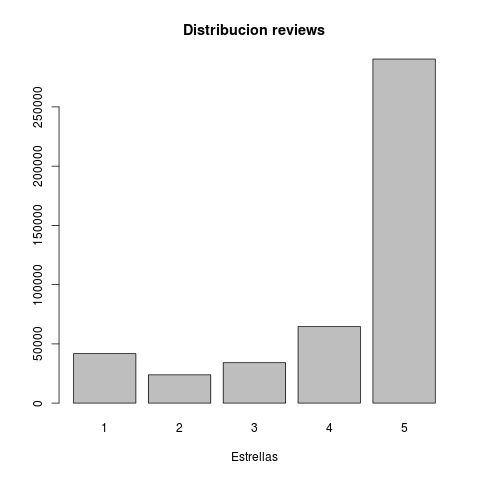
\includegraphics[width=1\linewidth]{Figures/dist_reviews.png}
\decoRule
\caption[Distribuci\'on de reviews]{Distribuci\'on de reviews con respecto a las clases.}
\label{fig:distribucion_reviews}
\end{figure}

La metodolog\'ia fue la siguiente:

\begin{itemize}
\setlength\itemsep{0em}
  \item Dividir los reviews de 5 estrellas en fracciones
  \item Por cada una de las fracciones
  \begin{itemize}
  \setlength\itemsep{0em}
    \item Mezclarla con los dem\'as reviews de 1-4 estrellas y entrenar la red con dicho set
  \end{itemize}
\end{itemize}

De esta forma se esperaba favorecer el aprendizaje sobre los reviews de valores menos frecuentes,
aunque los resultados mostraron que no hac\'ian una gran diferencia (en ning\'un caso hubo
siquiera una mejora).

% Chapter Template

\chapter{Modelo solo con RNN} % Main chapter title

\label{RNN} % Change X to a consecutive number; for referencing this chapter elsewhere, use \ref{ChapterX}

%----------------------------------------------------------------------------------------
%   SECTION 1
%----------------------------------------------------------------------------------------

\section{Primeros pasos}

Para estas pruebas, se utilizo en todo momento una red neural recurrente, proporcionada por el paquete NNET, para el lenguaje R.

Se comenzo realizando un pre procesado de los textos, como se había hablado en un inicio, en el cual se sacaron stopwords, se hizo un proceso de stemming y se dejo todo en un formato de texto plano.

Las primer idea, fue entrenar la red neuronal con una DTM TF, sin embargo, esto se vio rapidamente inviable.

La DTM completa poseía cerca de 10000 terminos, que no era un problema almacenarlos mientras pudieramos usar un formato de matriz hecho para matrices dispersas, sin embargo, para entrenar la red, se necesitaba una matriz en su formato tradicional.

El primer cambio realizado fue el mas trivial, quitar terminos cuya ocurrencia sea muy baja. Asi, se sacaron los terminos que aparecían con una frecuencia menor a 1 cada 100 documentos  y nos quedamos con aproximadamente 667 terminos.

Aún con esta cantidad, se tuvieron problemas de memoria, y la primer red neuronal fue entrenada con la mitad del set original, y utilizando un 80\% de los datos como train, y el resto como set.

El resultado fue cerca de un 14\% de precisión, la red neuronal no predecía.

\section{Primeras correcciones}

El error fue bastante evidente luego, nunca habíamos normalizado los datos. Decidimos entonces usar la normalización mas intuitiva. Aplicamos a todas las columnas la siguiente función:

\begin{equation}
z = \frac{x_{i}-min(x)}{max(x)-min(x)}
\end{equation}

Los resultados fueron igual de malos.

Entonces probamos otra una normalización gausseana, muchas veces llamada estandarización:

\begin{equation}
z = \frac{x_{i}-\mu(x)}{\sigma(x)}
\end{equation}

Y los resultados por primera vez fueron razonables. Redondeando los datos en el test se tuvo cerca de un 52\% de aciertos.

\section{Preparando para kaggle}

Para poder subir a Kaggle, necesitamos que nuestra red pueda predecir el test que tenemos. Sin embargo, se debe realizar la misma transformación a los datos que se le realizo al train. Para esto podíamos guardar los terminos y los datos de la media y el desvio estandar de cada de matriz, luego en el test quedarnos con esos terminos, y aplicar esa normalización. Siendo que solo nos interesa predecir un test, se decidio aprovechar para hacer todo esto, con el test y el train combinado.

Habiendo terminado eso, se subio la primer entrega a kaggle con un 1.15939 de error cuadrático medio.

\section{SVD}

Entrenar una red neuronal con una neurona, de la forma que veníamos haciendo era muy lento, y ocupaba mucho espacio en memoria. Por lo cual se decidio armar una SVD y quedarnos con los autovectores mas importante de la matriz u.

El primer inconveniente con esta idea, es que calcular la SVD, para la matriz DTM, excede nuestro poder computacional. Aún tirando terminos que se usan poco al principio. Si bien los métodos convenciales permiten cálcular menos vectores de U y de V, cálculan todos los autovalores. Y ahi se vuelve imposible 

Se recurrio entonces a otro algoritmo conocido como IRLBA, augmented implicitly restarted Lanczos bidiagonalization algorithm. Este nos permite cálcular nuestra SVD con la cantidad de autovectores y autovalores que necesitemos. Es extremedamente rápido para buscar los autovalroes mas grandes y sus autovectores asociados. Aunque es mas lento si se quiere computar toda la SVD, pero como eso nos era imposible, trabajamos con este método.

También posee la ventaja de poder reanudarse. Utilizando el resultado de la ultima iteración, se puede seguir calculando mas autovalores y autovectores de la SVD, por lo cual no se pierde el trabajo computado.

Cálculamos 170 autovectores y autovalores, con una noche completa de cálculo. Lo primero que hicimos fue ver como era la distribución de la energía, para ver cuanta información perderíamos al estimar con la SVD. Este fue el resultado:

\begin{figure}[h]
{
    \centering
    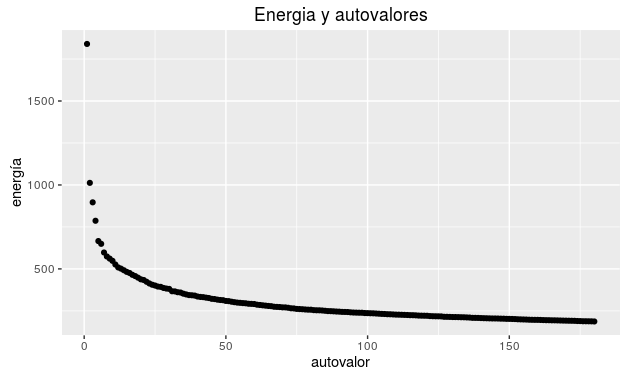
\includegraphics[width=1\linewidth]{Figures/svd.png}
}
Si lo ponemos en escala logaritmica\par\bigskip
{
    \centering
    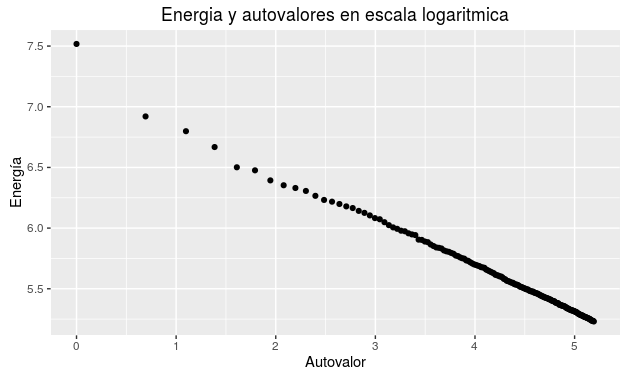
\includegraphics[width=1\linewidth]{Figures/svdLog.png}
}
\end{figure}

Lamentablemente, es una ley de potencias. La cola alargada que vemos, nos provoca que la energía comience a bajar muy de a poco. Y teniendo en cuenta que hay muchisimos terminos, el peso no es despreciable.

Aún así, siendo que de todas formas no podíamos utilizar todos los datos que teníamos, decidimos utilizar 50 columnas de la matriz u de la SVD para estimar los datos, y ver que sucede.

La velocidad a la que se entrena una red neuronal, y en consecuencia la cantidad de neuronas que podíamos utilizar, aumento considerablemente. Los resultados fueron un poco peores. 
Con una neurona y una capa, tal como fue el primero, se obtuvo en kaggle 1.32583 de RMSE. Recordamos que el original había sido 1.13817.

Sin embargo, aprovechando los nuevos tiempos de entrenamiento, se probo que pasaba si variabamos hiper parametros.

 
\section{Ajustando hiper parametrós}

Una primer prueba, solo por curiosidad, fue ver si había alguna diferencia cambiando de TF a IDF.

La red neuronal se entreno ligeramente mas rápido con IDF, y el resultado teniendo en cuenta la precisión fue:


TF - Precision en el Train: 55.3775 \%  
TF - Precision en el Test: 54.78959 \%

TF-IDF - Precision en el Train: 55.37\%  
TF-IDF  - Precision en el Test: 54.72912 \%

El cambio fue minimo. Se continuo usando TF que fue ligeramente superior.

Pasadas nuestras pequeñas pruebas, se planteo que había que automatizar la forma de ajustar hiper parametros. Y realizar una comparación mejor, que redondear los resultados.

Para esto utilizamos la librería Caret, y con ella, continuamos utilizando el mismo modelo. Ahora entrenamos con un two fold cross validation, y comparando con el error cuadratico medio. Trabajamos con una capa, y variamos la cantidad de neuronas y el decay. Para generar redes mas rápido, utilizamos una muestra del set. Al final entrenaremos con todo el set.

Elegimos two fold cross validation, porque si bien aumentamos la velocidad a la que calculamos una red neuronal, sigue sin ser despreciable el tiempo utilizado, mas cuando ahora la empezamos a complejizar. Por otro lado, configuramos el sistema para que compute distintas redes en diferentes nucleos y acelerar el proceso. También redujimos a un 20\% el set de entrenamiento, para poder computar más rápidamente las redes.

Este fue el primer resultado:

\begin{center}
    \begin{tabular}{| l | l | l | l |}
    \hline
    decay & size & RMSE & Rsquared \\ \hline
    0.000 & 1 & 1.164061 & 0.2123402 \\ 
    0.000 & 2 & 1.144628 & 0.2383667  \\
    0.000 & 10 & 1.145871 & 0.2401054  \\
    0.001 & 1 & 1.153106 & 0.2270361  \\
    0.001 & 2 & 1.155142 & 0.2251961  \\
    0.001 & 10 & 1.131491 & 0.2577052  \\
    0.010 & 1 & 1.152959 & 0.2272637  \\
    0.010 & 2 & 1.135215 & 0.2507921  \\
    0.010 & 10 & 1.131509 & 0.2572446  \\
    \hline
    \end{tabular}
\end{center}

Vemos que a medida que cuando aumenta la cantidad de neuronas el resultado en general mejora. Por otro lado, tener un poco de decay ayuda. Si bien el mejor resultado lo obtuvimos con un decay de 0.001, es en el caso de un decay de 0.01 donde siempre mejora el resultado, para todo tamaño de red. Y los valores son similares.

Agregamos entonces dos pruebas mas, con mas neuronas, y observamos que empeoro.

\begin{center}
    \begin{tabular}{| l | l | l | l |}
    \hline
    decay & size & RMSE & Rsquared \\ \hline
    0.01 & 20 & 1.136187 & 0.2557508 \\
    0.01 & 50 & 1.171565 & 0.2322588 \\
    \hline
    \end{tabular}
\end{center}

Entrenando conla muestra el resultado en kaggle fue de un RMSE de 1.26806. Y al entrenar con todo el train disponible llegamos a 1.20078. Un resultado que se empieza a acercar al primero.


%----------------------------------------------------------------------------------------
%	BIBLIOGRAPHY
%----------------------------------------------------------------------------------------

\printbibliography[heading=bibintoc]

%----------------------------------------------------------------------------------------

\end{otherlanguage}
\end{document}
